\chapter{Scan Matching: Fitting Clouds Together}

\section{The puzzle-piece idea}
\begin{kid}
Draw a shape on a see-through sheet. Your friend draws the same shape on another sheet, but a little shifted and turned. Lay the sheets on top of each other and slide and twist the top one until the drawings line up perfectly. How far you slid and twisted it tells you how your friend's sheet was placed! A LiDAR does this with two scans: sliding and twisting the new scan until it lines up with the old one tells it how far the car moved.
\end{kid}

\begin{eng}
Scan matching (registration) finds the rigid transform $(\vect R,\vect t)$ that best aligns a source cloud $\{\vect p_i\}$ to a target cloud or map $\{\vect q_i\}$. Matching each new scan to the previous one gives \emph{scan-to-scan} odometry; matching to an accumulated local map gives \emph{scan-to-map} odometry, which drifts less. LIO-SAM matches each new keyframe to a local map built from its recent ``sub-keyframes'' (Module 12). The answer becomes a measurement (a factor) of how the vehicle moved.
\end{eng}

\section{Iterative Closest Point (ICP)}
\fig[1.0]{icp_iters}{A real ICP run: pair each red point with its nearest blue point, solve the best fit, move, repeat.}

\begin{keyeq}{The ICP objective}
\[ \min_{\vect R,\vect t}\ E=\sum_{i=1}^{N}\big\|\vect R\vect p_i+\vect t-\vect q_{c(i)}\big\|^2 \]
\begin{symbols}
$\vect p_i$ & point $i$ of the new (source) scan & m\\
$\vect q_{c(i)}$ & its corresponding (closest) point in the target & m\\
$c(i)$ & the correspondence: which target point is paired with $\vect p_i$ & ---\\
$\vect R,\vect t$ & rotation and translation being solved for & ---, m\\
$\|\cdot\|^2$ & squared distance & m$^2$\\
$E$ & total squared misfit (least-squares cost) & m$^2$\\
\end{symbols}
\end{keyeq}

The algorithm alternates two easy problems:
\begin{enumerate}
\item \textbf{Associate:} for the current guess, pair every source point with its nearest target point (a k-d tree makes this fast).
\item \textbf{Solve:} with pairs fixed, find the best $(\vect R,\vect t)$ in closed form (below).
\item \textbf{Apply} the transform and \textbf{repeat} until the cost stops decreasing.
\end{enumerate}
ICP converges to the nearest local minimum, so it needs a good starting guess --- which the IMU provides.

\begin{keyeq}{Closed-form best fit (Arun/Horn/Umeyama)}
\[ \bar{\vect p}=\tfrac1N\textstyle\sum\vect p_i,\quad \bar{\vect q}=\tfrac1N\sum\vect q_i,\quad
\vect W=\sum(\vect p_i-\bar{\vect p})(\vect q_i-\bar{\vect q})^{\mathsf T}=\vect U\boldsymbol\Sigma\vect V^{\mathsf T},\quad
\vect R=\vect V\vect U^{\mathsf T},\quad \vect t=\bar{\vect q}-\vect R\bar{\vect p} \]
In 2-D this reduces to \ $\displaystyle \theta=\operatorname{atan2}\Big(\textstyle\sum(p'_xq'_y-p'_yq'_x),\ \sum(p'_xq'_x+p'_yq'_y)\Big)$.
\begin{symbols}
$\bar{\vect p},\bar{\vect q}$ & centroids (average points) of the two sets & m\\
$\vect p',\vect q'$ & points with their centroid subtracted (``centered'') & m\\
$\vect W$ & cross-covariance matrix of the centered sets & m$^2$\\
$\vect U,\boldsymbol\Sigma,\vect V$ & singular value decomposition of $\vect W$; if $\det(\vect V\vect U^{\mathsf T})=-1$ flip the last column of $\vect V$ to avoid a mirror image & ---\\
\end{symbols}
\end{keyeq}

\begin{minipage}[t]{0.55\linewidth}
\begin{worked}{best fit of four matched points}
\textbf{Given:} source $\vect p_{1..4}=(0,0),(2,0),(2,1),(0,3)$; target $\vect q_{1..4}=(1.000,0.500)$, $(2.970,0.847)$, $(2.796,1.832)$, $(0.479,3.454)$, already paired.
\step{Step 1 --- centroids} $\bar{\vect p}=(1,1)$;\ $\bar{\vect q}=(1.811,1.658)$
\step{Step 2 --- center and sum} (table below)
\end{worked}
\end{minipage}\hfill
\begin{minipage}[t]{0.42\linewidth}\vspace{0pt}
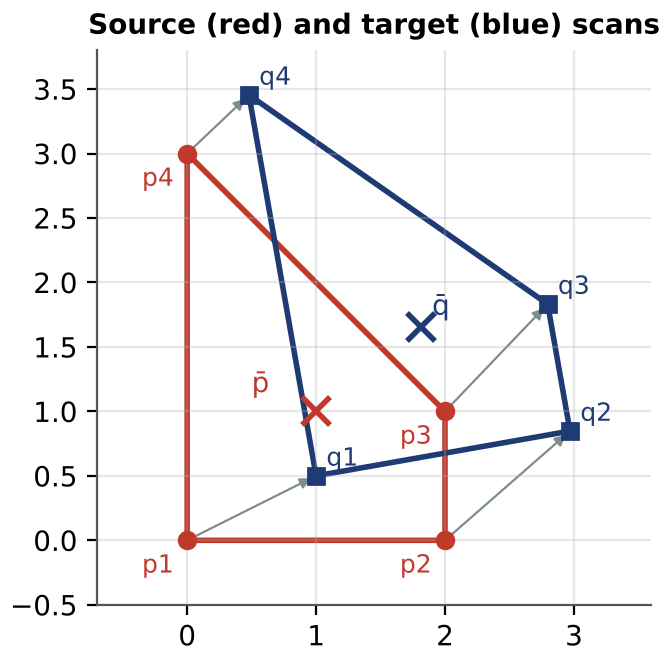
\includegraphics[width=\linewidth]{icp4}
\end{minipage}

\begin{center}\small
\begin{tabular}{rrrrrr}\toprule
$p'_x$&$p'_y$&$q'_x$&$q'_y$&$p'_xq'_x+p'_yq'_y$&$p'_xq'_y-p'_yq'_x$\\\midrule
$-1$&$-1$&$-0.811$&$-1.158$&1.970&0.347\\
$1$&$-1$&$1.158$&$-0.811$&1.970&0.347\\
$1$&$0$&$0.985$&$0.174$&0.985&0.174\\
$-1$&$2$&$-1.332$&$1.796$&4.924&0.868\\\midrule
&&&\textbf{Sum}&\textbf{9.848}&\textbf{1.736}\\\bottomrule
\end{tabular}\end{center}

\begin{worked}{(continued)}
\step{Step 3 --- rotation} $\theta=\operatorname{atan2}(1.736,\ 9.848)=10.00^\circ$
\step{Step 4 --- translation} $\vect t=\bar{\vect q}-\vect R\bar{\vect p}$:\ $\vect R\bar{\vect p}=(0.9848-0.1736,\ 0.1736+0.9848)=(0.811,\ 1.158)$;\ $\vect t=(1.811-0.811,\ 1.658-1.158)=(1.000,\ 0.500)$
\step{Step 5 --- check with SVD} $\vect W=\begin{psmallmatrix}4.287&-1.275\\-3.012&5.562\end{psmallmatrix}$ gives $\vect V\vect U^{\mathsf T}=\begin{psmallmatrix}0.985&-0.174\\0.174&0.985\end{psmallmatrix}$ $=\vect R(10^\circ)$ \checkmark
\result{the second scan is the first rotated 10° and shifted (1.0, 0.5) m --- exactly how the target was made. In real ICP the pairs are only guesses, so steps 1--5 repeat.}
\end{worked}

\section{Better cost functions: point-to-plane and NDT}
\fig[0.95]{p2plane}{Point-to-point pulls toward sample points; point-to-plane only penalizes the gap normal to the surface.}

\begin{keyeq}{Point-to-plane ICP}
\[ E=\sum_i\Big(\big(\vect R\vect p_i+\vect t-\vect q_i\big)\cdot\vect n_i\Big)^2 \]
\begin{symbols}
$\vect n_i$ & unit normal of the target surface at $\vect q_i$ & ---\\
$(\cdot)\cdot\vect n_i$ & dot product: keeps only the part of the gap perpendicular to the surface & m\\
\end{symbols}
\end{keyeq}

\fig[0.55]{ndt}{The Normal Distributions Transform summarizes each grid cell by a mean and covariance.}
\begin{eng}
\textbf{NDT} (Normal Distributions Transform) divides the target into voxels and fits each with a Gaussian (mean $\boldsymbol\mu_k$, covariance $\boldsymbol\Sigma_k$). The source is scored by $\sum_i\exp\!\big(-\tfrac12(\vect x_i-\boldsymbol\mu_k)^{\mathsf T}\boldsymbol\Sigma_k^{-1}(\vect x_i-\boldsymbol\mu_k)\big)$ with $\vect x_i=\vect R\vect p_i+\vect t$, and maximized. No nearest-neighbor search is needed, it is smooth, and it is widely used in automotive localization. \textbf{Generalized ICP} (GICP) blends both ideas by modeling local surface covariances on both clouds.
\end{eng}

\section{Feature-based matching (LOAM and LIO-SAM)}
\fig[0.72]{loam}{Points on sharp corners become edge features; points on smooth surfaces become planar features.}

\begin{kid}
Instead of matching every single dot, look for the \emph{special} ones: sharp corners (like the corner of a box) and flat sides (like a table top). Corners are easy to recognize and flat sides are easy to slide against. Matching only these is much faster.
\end{kid}

\begin{keyeq}{Roughness (curvature) score}
\[ c_i=\frac{1}{|S|\cdot\rho_i}\ \Big|\sum_{j\in S}(\rho_j-\rho_i)\Big| \]
\begin{symbols}
$\rho_i$ & range of point $i$ along one scan line & m\\
$S$ & its neighbors on the same scan line ($|S|$ = how many, e.g.\ 5 each side) & ---\\
$c_i$ & roughness: large $\Rightarrow$ edge feature; small $\Rightarrow$ planar feature & ---\\
\end{symbols}
(Simplified range form; LOAM uses the same expression with 3-D point vectors.)
\end{keyeq}

\begin{worked}{edge or plane?}
\textbf{Given:} two neighbors each side ($|S|=4$).
\step{Flat wall} ranges $10.00,\ 10.01,\ \underline{10.00},\ 9.99,\ 10.00$: sum of differences $=0+0.01-0.01+0=0$ $\Rightarrow c=0$ \quad\textbf{planar}
\step{Corner} ranges $10.0,\ 10.0,\ \underline{8.0},\ 8.0,\ 8.0$: sum $=2+2+0+0=4$ $\Rightarrow c=4/(4\times8)=0.125$ \quad\textbf{edge}
\result{thresholds (e.g.\ $c>0.1$ edge, $c<0.1$ plane in LOAM's default) sort the points.}
\end{worked}

\subsection{Distances to edges and planes (LIO-SAM eqs.\ 10--11)}
\fig[0.92]{edgeplane}{An edge feature is compared with a line through two map points; a planar feature with a plane through three.}

\begin{keyeq}{Point-to-line and point-to-plane distances}
\[ d_e=\frac{\big\|(\vect p-\vect a)\times(\vect p-\vect b)\big\|}{\|\vect a-\vect b\|}\qquad\qquad
d_p=\frac{\big|(\vect p-\vect u)\cdot\big((\vect u-\vect v)\times(\vect u-\vect w)\big)\big|}{\big\|(\vect u-\vect v)\times(\vect u-\vect w)\big\|} \]
\begin{symbols}
$\vect p$ & a feature point of the new scan, transformed into the map frame with the current guess & m\\
$\vect a,\vect b$ & two map points defining the matching edge line ($\vect p^e_{i,u},\vect p^e_{i,v}$ in the paper) & m\\
$\vect u,\vect v,\vect w$ & three map points defining the matching planar patch & m\\
$\times$ & cross product (Module 2): its length is a parallelogram area; area $\div$ base = height = distance & ---\\
$(\vect u-\vect v)\times(\vect u-\vect w)$ & a vector normal to the plane & m$^2$\\
\end{symbols}
\end{keyeq}

\begin{worked}{edge and plane distances}
\step{Edge} $\vect a=(0,0,0)$, $\vect b=(2,0,0)$, $\vect p=(1,0.6,0.8)$.
$\vect p-\vect a=(1,0.6,0.8)$, $\vect p-\vect b=(-1,0.6,0.8)$; cross $=(0.6\cdot0.8-0.8\cdot0.6,\ 0.8\cdot(-1)-1\cdot0.8,\ 1\cdot0.6-0.6\cdot(-1))=(0,-1.6,1.2)$; length $=\sqrt{2.56+1.44}=2.0$; divide by $\|\vect a-\vect b\|=2$: $d_e=1.0$ m.
\step{Plane} $\vect u=(0,0,0)$, $\vect v=(1,0,0)$, $\vect w=(0,1,0)$, $\vect p=(0.3,0.4,0.12)$. Normal $=(\vect u-\vect v)\times(\vect u-\vect w)=(-1,0,0)\times(0,-1,0)=(0,0,1)$; $d_p=|(0.3,0.4,0.12)\cdot(0,0,1)|/1=0.12$ m.
\result{LIO-SAM then finds the pose that minimizes $\sum d_e+\sum d_p$ over all features using the Gauss--Newton method.}
\end{worked}

\begin{eng}
\textbf{Gauss--Newton in one paragraph.} Stack all distances into a residual vector $\vect d(\vect x)$ that depends on the 6-DOF pose $\vect x$. Linearize: $\vect d(\vect x+\delta\vect x)\approx\vect d+\vect J\delta\vect x$, where $\vect J$ is the Jacobian. Setting the derivative of $\|\vect d+\vect J\delta\vect x\|^2$ to zero gives the \emph{normal equations} $\vect J^{\mathsf T}\vect J\,\delta\vect x=-\vect J^{\mathsf T}\vect d$ --- exactly the normal equations of a survey least-squares adjustment. Solve, update $\vect x\leftarrow\vect x+\delta\vect x$, repeat until $\delta\vect x$ is tiny.
\end{eng}

\section{When matching fails: the hallway effect}
\fig[0.98]{hallway}{In a featureless corridor the matching error has a flat valley along the corridor --- any forward shift fits equally well.}

\begin{eng}
Scan matching can only measure motion in directions where geometry changes. In a long uniform corridor, tunnel, or a highway with continuous barriers, the cost is flat along the axis, $\vect J^{\mathsf T}\vect J$ is nearly singular in that direction, and the estimate is free to stretch or shrink. Mathematically, the smallest eigenvalue of $\vect J^{\mathsf T}\vect J$ is near zero; some systems monitor this ``degeneracy'' and down-weight LiDAR along that axis. Surveyors recognize this as a traverse with poor geometry in one direction.
\end{eng}

\begin{tip}
In corridors: add control or targets along the length, walk/drive both directions, include side rooms or cross-ties to create unique geometry, place temporary objects (cones, boxes) if needed, and always check along-track distances against a taped or total-station measurement.
\end{tip}

\begin{tryit}
\textbf{11.1} Source points $(0,0),(1,0)$ match target points $(2,1),(2,2)$. Find $\theta$ and $\vect t$ by the closed form.\\
\textbf{11.2} Distance from $\vect p=(3,4,5)$ to the line through $(0,0,0)$ and $(0,0,10)$?\\
\textbf{11.3} (Simple) Why is it hard to tell how far you have walked in a long, plain hallway with your eyes half-closed?
\end{tryit}

\sources{Besl \& McKay (1992), \emph{IEEE PAMI} 14(2); Arun, Huang \& Blostein (1987), \emph{IEEE PAMI} 9(5); Segal \emph{et al.}\ (2009), Generalized-ICP; Biber \& Stra{\ss}er (2003), NDT; Zhang \& Singh (2017), LOAM, \emph{Autonomous Robots} 41(2); Shan \emph{et al.}\ (2020), eqs.\ (10)--(11).}
